% Chapter 4, Section 2: Gradient-Based Optimization

\section{Gradient-Based Optimization \difficultyInline{beginner}}
\label{sec:gradient-optimization}

Gradient-based optimization is the fundamental method for training deep learning models, using the mathematical concept of gradients to iteratively find optimal parameters that minimize loss functions through careful navigation of high-dimensional parameter spaces.

\subsection{Intuition: Finding the Bottom of a Hill}

Imagine you're hiking in foggy mountains and need to find the lowest point in a valley. You can't see far ahead, but you can feel the slope under your feet. The steepest downward direction tells you which way to walk to get lower. This is exactly what gradient descent does, where the mountain represents the loss function we want to minimize, your position represents the current parameter values, the slope represents the gradient (direction of steepest increase), and your steps represent parameter updates. Most deep learning algorithms involve optimization, which is the process of finding parameters that minimize or maximize an objective function, making gradient descent the cornerstone of neural network training.

\subsection{Gradient Descent}

For a function $f(\vect{\theta})$, \textbf{gradient descent} updates parameters as:

\begin{equation}
\vect{\theta}_{t+1} = \vect{\theta}_t - \alpha \nabla_{\vect{\theta}} f(\vect{\theta}_t)
\end{equation}

where $\alpha > 0$ is the \textbf{learning rate}.

\subsubsection{Example: Gradient Descent in 2D}

Consider minimizing $f(x, y) = x^2 + 2y^2$ starting from $(3, 3)$:

\begin{figure}[h]
\centering
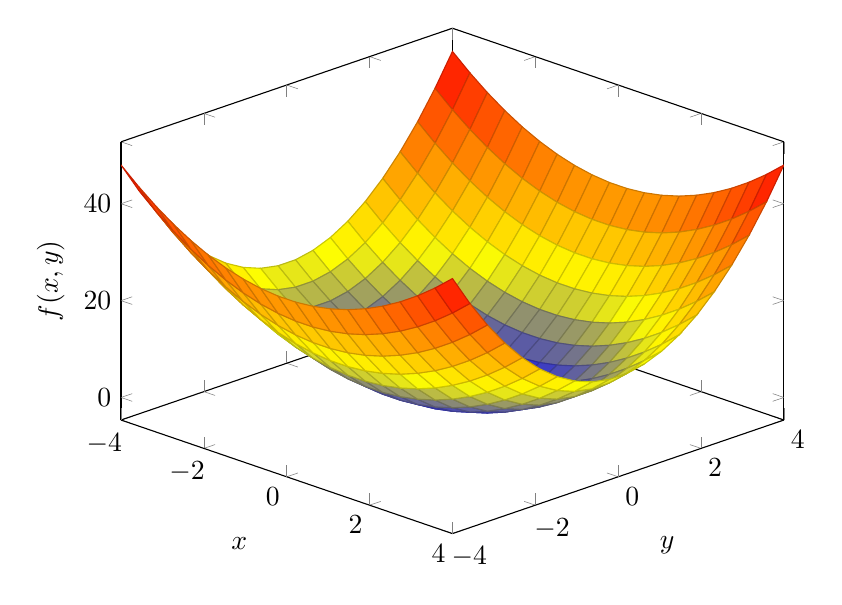
\begin{tikzpicture}
\begin{axis}[
    xlabel={$x$},
    ylabel={$y$},
    zlabel={$f(x,y)$},
    width=10cm,
    height=8cm,
    view={45}{30}
]
\addplot3[
    surf,
    domain=-4:4,
    domain y=-4:4,
    samples=20
] {x^2 + 2*y^2};
\end{axis}
\end{tikzpicture}
\caption{Contour plot of $f(x,y) = x^2 + 2y^2$ showing gradient descent path}
\label{fig:gradient-descent-2d}
\end{figure}

The gradient is $\nabla f = [2x, 4y]$. Starting from $(3, 3)$ with learning rate $\alpha = 0.1$:
\begin{align}
\nabla f(3, 3) &= [6, 12] \\
(x_1, y_1) &= (3, 3) - 0.1[6, 12] = (2.4, 1.8) \\
\nabla f(2.4, 1.8) &= [4.8, 7.2] \\
(x_2, y_2) &= (2.4, 1.8) - 0.1[4.8, 7.2] = (1.92, 1.08)
\end{align}

\subsection{Jacobian and Hessian Matrices}

The \textbf{Jacobian matrix} contains all first-order partial derivatives. For $\vect{f}: \mathbb{R}^n \to \mathbb{R}^m$:

\begin{equation}
\mat{J}_{ij} = \frac{\partial f_i}{\partial x_j}
\end{equation}

The \textbf{Hessian matrix} contains second-order derivatives:

\begin{equation}
\mat{H}_{ij} = \frac{\partial^2 f}{\partial x_i \partial x_j}
\end{equation}

The Hessian characterizes the local curvature of the function.

\subsection{Taylor Series Approximation}

Near point $\vect{x}_0$, we can approximate $f(\vect{x})$ using Taylor series:

\begin{equation}
f(\vect{x}) \approx f(\vect{x}_0) + (\vect{x} - \vect{x}_0)^\top \nabla f(\vect{x}_0) + \frac{1}{2}(\vect{x} - \vect{x}_0)^\top \mat{H}(\vect{x}_0) (\vect{x} - \vect{x}_0)
\end{equation}

This provides insight into optimization behavior.

\begin{example}[Taylor Series for $f(x) = e^x$ around $x_0 = 0$]
For the exponential function $f(x) = e^x$, we can compute the Taylor series expansion around $x_0 = 0$:

Since all derivatives of $e^x$ are $e^x$, and $e^0 = 1$, we have:
\begin{align}
f(0) &= 1 \\
f'(0) &= 1 \\
f''(0) &= 1 \\
f'''(0) &= 1 \\
&\vdots
\end{align}

The Taylor series expansion is:
\begin{equation}
e^x \approx 1 + x + \frac{x^2}{2!} + \frac{x^3}{3!} + \frac{x^4}{4!} + \cdots
\end{equation}

For small values of $x$, we can use the first few terms:
\begin{itemize}
    \item Linear approximation: $e^x \approx 1 + x$
    \item Quadratic approximation: $e^x \approx 1 + x + \frac{x^2}{2}$
    \item Cubic approximation: $e^x \approx 1 + x + \frac{x^2}{2} + \frac{x^3}{6}$
\end{itemize}

For example, $e^{0.1} \approx 1 + 0.1 + \frac{0.01}{2} = 1.105$, which is very close to the true value of approximately $1.1052$.
\end{example}

\subsection{Critical Points}

Critical points are locations where the gradient is zero, representing different types of terrain features in the optimization landscape. A local minimum is like the bottom of a bowl where you can't go lower in any direction, a local maximum is like the top of a hill where you can't go higher in any direction, and a saddle point is like a mountain pass where you can go down in some directions and up in others. At a critical point, $\nabla f(\vect{x}) = \boldsymbol{0}$, and the Hessian matrix determines the nature of the critical point: a local minimum occurs when the Hessian is positive definite, a local maximum occurs when the Hessian is negative definite, and a saddle point occurs when the Hessian has both positive and negative eigenvalues.

\begin{figure}[h]
\centering
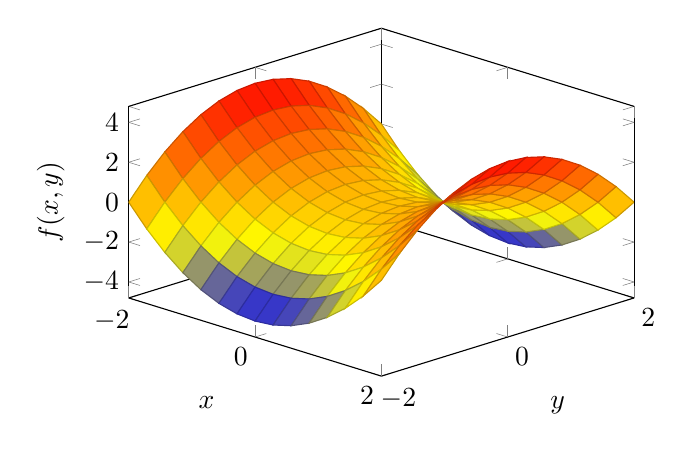
\begin{tikzpicture}
\begin{axis}[
    xlabel={$x$},
    ylabel={$y$},
    zlabel={$f(x,y)$},
    width=8cm,
    height=6cm,
    view={45}{30}
]
\addplot3[
    surf,
    domain=-2:2,
    domain y=-2:2,
    samples=15
] {x^2 - y^2};
\end{axis}
\end{tikzpicture}
\caption{Example of a saddle point: $f(x,y) = x^2 - y^2$}
\label{fig:saddle-point}
\end{figure}

Deep learning often encounters saddle points rather than local minima in high dimensions.

\subsection{Directional Derivatives}

The directional derivative in direction $\vect{u}$ (with $\|\vect{u}\| = 1$) is:

\begin{equation}
\frac{\partial}{\partial \alpha} f(\vect{x} + \alpha \vect{u}) \bigg|_{\alpha=0} = \vect{u}^\top \nabla f(\vect{x})
\end{equation}

To minimize $f$, we move in the direction $\vect{u} = -\frac{\nabla f(\vect{x})}{\|\nabla f(\vect{x})\|}$.
